\section{INTRODUCTION}

Unlike in General Relativity, the notion of \textbf{time} in Quantum Mechanics is considered a parameter, and no adequate \textbf{Time Operator} has been produced since physicists first started pondering the question in 1939 (see appendix \ref{ap:time_context} for a deeper treatment). Canonical quantum formalism seems to be particularly concerned with \textbf{measurement outcomes}, with less interest in the \textit{journey} that a particle takes from its \textit{conception} to its measurement. For instance, the famous interference pattern produced in the dual slit experiment is incredibly well described and predicts experimental outcomes adequately. To get a fuller picture of such an elementary experiment, however, the idea of "time of flight" of a quantum particle is required. The central question in this study resounds as follows:
\begin{center}
    \textit{When will a detector click?}
\end{center}
The answer to this question is answered by the \textbf{Arrival Time Distribution} of a quantum system at some detector location or surface. For trivial systems with no barriers or scattering potentials, the mean arrival time can be estimated semiclassically as $\tau_{arrival} \simeq \nicefrac{L}{\langle v \rangle}$, with $\langle v\rangle=\nicefrac{\hat{p}}{m}$, but this approach breaks for even the most basic potentials and barriers. Canonical quantum mechanics can't answer this question, but in Bohmian Mechanics, an alternative formulation of quantum mechanics which holds the same predictive power as canonical formalisms, the arrival time \textit{is} calculable and mainly justified by the theory's existence of \textbf{Bohmian trajectories}. In experiment, the arrival time has been measured for the double slit experiment using He atoms \cite{kurtsiefer1997measurement}, whose results have been modelled and numerically reproduced using Bohmian Theory \cite{DAS2025170054} \cite{das2022double}. An image of both can be found in figure \ref{fig:doubleslit_main_results}. A clear "fanning out" of the arrival time has been observed and predicted, which after further analysis was due to an inherent uncertainty on the initial momentum $p_0$ of shot particles through the dual slits. This gave rise to the idea of conceiving a physically realizable experiment (using ultracold atoms and neutrons like in \cite{vincent2009quantumtrampolineultracoldatoms}, \cite{Debu:2861358}, \cite{Zakharov_2016}, and \cite{KULIN201538}) for which the initial conditions can be controlled exactly, allowing precise prediction and subsequent measurement of arrival time distributions in quantum mechanics.
The answer to this question is answered by the \textbf{Arrival Time Distribution} of a quantum system at some detector location or surface. For trivial systems with no barriers or scattering potentials, the arrival time can be adequately described using semi-classical methods (via $m\langle v\rangle=\hat{H} \psi$). Canonical quantum mechanics can't answer this question, but in Bohmian Mechanics, an alternative formulation of quantum mechanics which holds the same predictive power as canonical formalisms, the arrival time \textit{is} calculable and mainly justified by the theory's existence of \textbf{Bohmian trajectories}. In experiment, the arrival time has been measured for the double slit experiment using He atoms \cite{kurtsiefer1997measurement}, whose results have been modelled and numerically reproduced using Bohmian Theory \cite{DAS2025170054} \cite{das2022double}. An image of both can be found in figure \ref{fig:doubleslit_main_results}. A clear "fanning out" of the arrival time has been observed and predicted, which after further analysis was due to an inherent uncertainty on the initial momentum $p_0$ of shot particles through the dual slits. This gave rise to the idea of conceiving a physically realizable experiment (using ultracold atoms (neutrons) like in \cite{vincent2009quantumtrampolineultracoldatoms}, \cite{Debu:2861358}, \cite{Zakharov_2016}, and \cite{KULIN201538}) for which the initial conditions can be controlled exactly, allowing precise prediction and subsequent measurement of arrival time distributions in quantum mechanics.

\begin{figure}
    \centering
    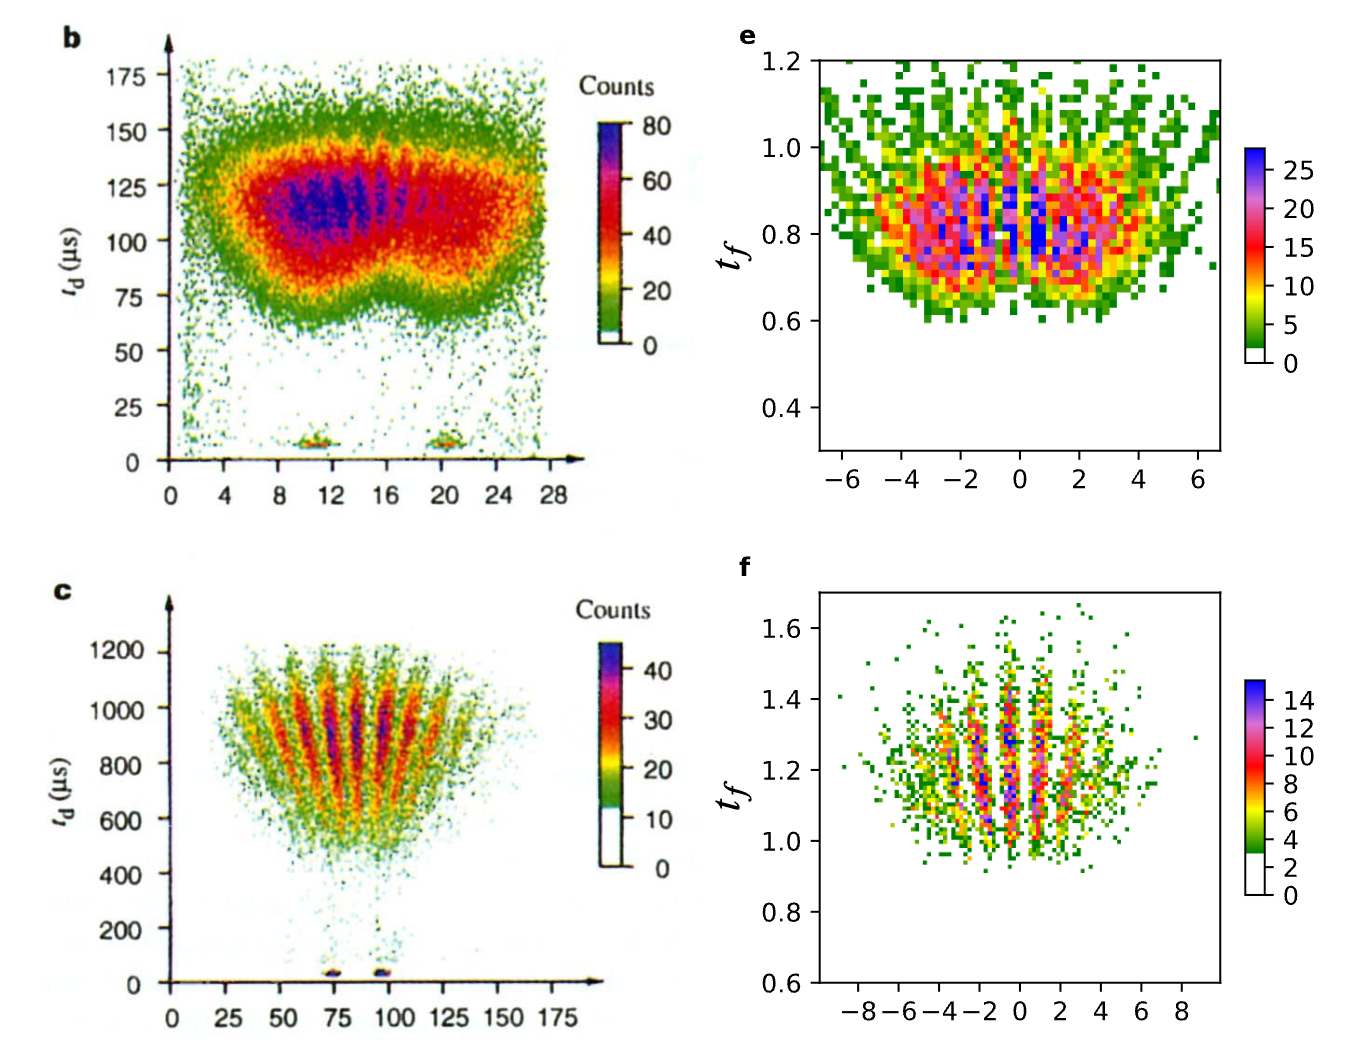
\includegraphics[width=1\linewidth]{Figures/bohmiandubbleslitexp.png}
    \caption{Figure showing arrival times of He atoms shod through a dual slit (left), and numerical predictions made using a Bohmian mechanics \cite{DAS2025170054}}
    \label{fig:doubleslit_main_results}
\end{figure}

One such proposed experiment by our research group is putting a quantum particle at rest in free fall. The particle would fall onto a barrier, and a detector would be put below the barrier. The detector will measure the arrival time of the tunnelled component. Since the barrier will reflect a portion of the wave function back up, that portion would inevitably fall back down again due to the linear gravitation potential, giving rise to quantum mechanical arrival time distributions to be studied both experimentally, and theoretically.
\\\\
\fbox{%
  \begin{minipage}{0.46\textwidth}
  Arrival time distributions of quantum particles falling onto Gaussian barriers under free fall has not yet been studied in literature, making this study an initial theoretical analysis of such setups.
  \end{minipage}%
}

The second part of this study focuses on \textbf{tunnelling time} of free-falling spin-$\frac{1}{2}$ particles onto magnetic Gaussian barriers, comparing Bütticker's Larmor Clock in the low magnetic regime with predictions made with Bohmian Formalism. A more thorough explication of the arrival time and tunnelling time in context of literature can be found in appendix \ref{ap:arrivaltimetunnelingtime}.
\begin{figure}
    \centering
    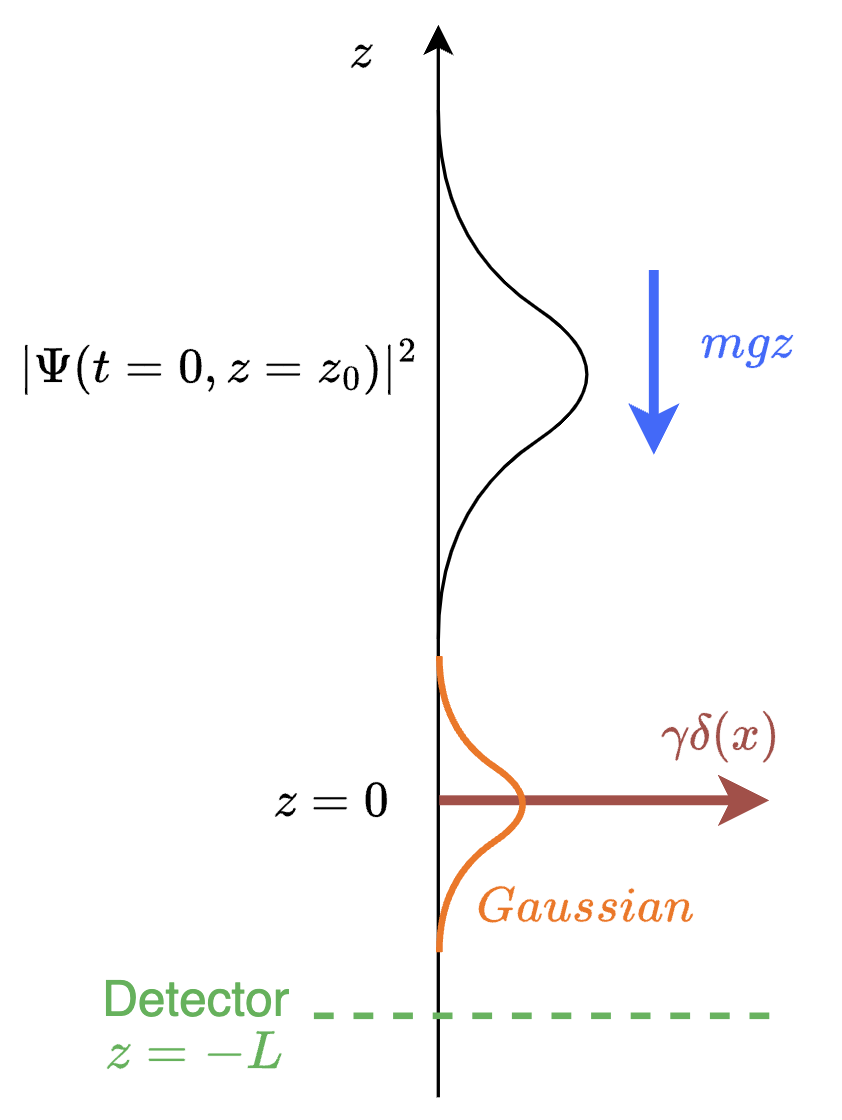
\includegraphics[width=\linewidth]{Figures/1d_setup_barrier.png}
    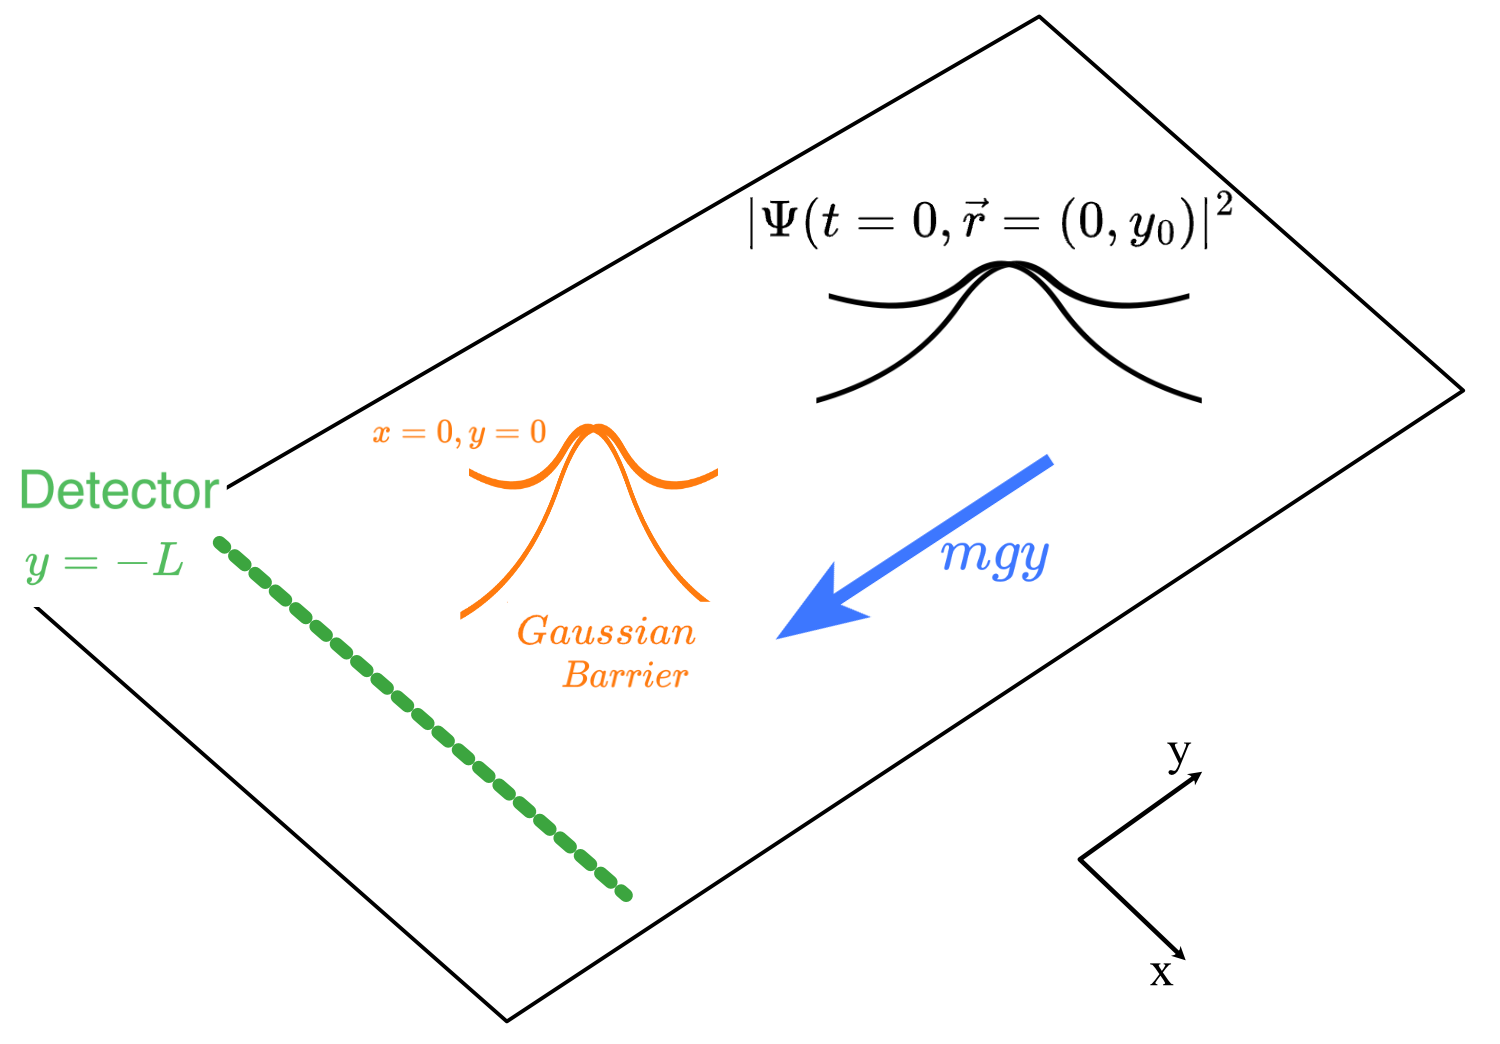
\includegraphics[width=1\linewidth]{Figures/2d_setup_barrier.png}
    \caption{Setup of Gaussian Particle Falling onto a barrier in 1 dimension, with a detector present at $z=-L$. In this study, barriers of the delta type $\gamma \delta$ and Gaussian types are considered. The 2D setup is of similar nature to the 1D experiment, where the barrier represents a uniform magnetic field of a Gaussian amplitude profile pointing in the z direction.}
    \label{fig:1d_setup}
\end{figure}

